\documentclass{article}
\usepackage[utf8]{inputenc}
\usepackage{hyperref}
\usepackage{amsmath}
\usepackage{amsfonts}
\usepackage{graphicx}


\title{SPhO Ten Year Series (TYS) with Solutions: 2012 Questions}
\author{
    Solutions available on Victoris\\
    \texttt{victoris.org}
    % new collaborators add your name and contact here!
}

\date{\today}

\begin{document}
\maketitle

\section{2012}

\subsection{Question 1}
1. A platform scale is calbrated to indicate the mass in $\mathrm{kg}$ of an object placed on it. Particles fall from a height of $3.5 \mathrm{~m}$ and collide with the balance pan of the scale. Assuming that the collisions are elastic and that the particles rebound upwards with the same speed they had before hitting the pan, determine the average scale reading if each particle has mass $110 \mathrm{~g}$ and collisions occur at the rate of $42 \mathrm{~s}^{-1}$. [8] \\

\subsection{Question 2}
2. A collection of $N$ identical blocks, each of mass $M$, are connected by unstretchable ropes of negligible mass. The blocks are on a horizontal surface. An external force $F_{0}$ acts on Block 1, pulling it horizontally to the right with constant velocity. What is the tension in the rope connecting Block $n$ to Block $n+1$, if
\begin{figure}
	\centering
	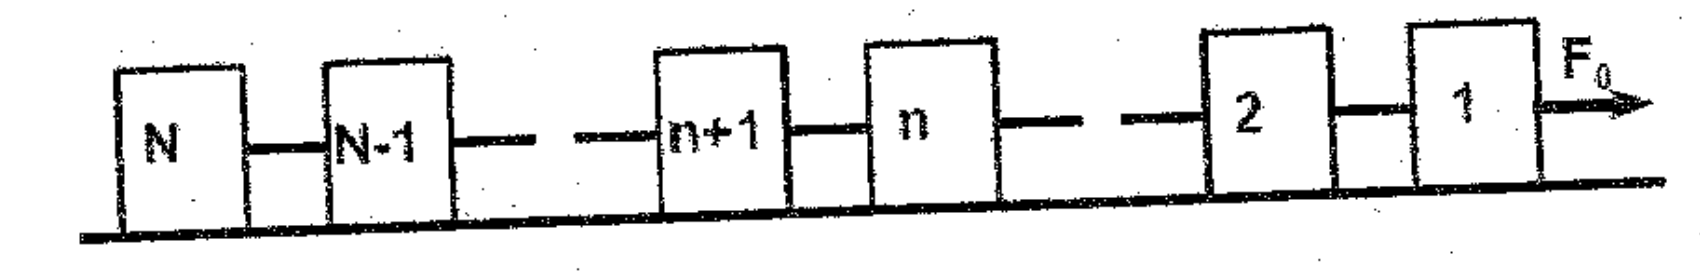
\includegraphics[width=0.7\linewidth]{spho_book_TYS_images/2012q1.png}
	\caption{$N$ identical blocks}
\end{figure}
(i) There is no friction between the blocks and the surface? [3] \\
(ii) The coefficient of kinetic friction between each block and the surface is $\mu_{k}$? ( $F_{0}$ large enough to accelerate the blocks despite the friction.) [5] \\

\subsection{Question 3}
3. A pendulum bob is constructed by taking a thin, uniform-density circular ring of mass $M$ and radius $R$ and affixing a straight, thin, uniform density rod of mass ${m}$ and length $2 R$ across its diameter as shown in the diagram. The pendulum hangs in a vertical plane from a frictionless pivot that can be attached to the ring at any point. The pivot allows the bob to swing either in the plane of the bob or in the plane perpendicular to the bob. Assume the angular amplitude is small.

(i) What swinging configurations givd the maximum period? [4]
(ii) What swinging configurations give the minimum period? [4]
(iii) Find the ratio of the maximum period to the minimum period. [2]

\subsection{Question 4}
4. The distance from the centre of the Earth to the poles is $21 \mathrm{~km}$ shorter than the radius of the equator. A one second pendulum is taken from the equator (at sea level) to the North Pole. Make a rough estimate of its change in period. You may assume for the purposes of your calculation that the Earth has a constant density. [6]

\subsection{Question 5}
5. A square lattice of identical resistances (1 ohm along each edge) is wrapped around an infinite cylinder in such a way that $N$ resistances are placed along the cross sectional circle of the cylinder. What are the resultant resistances between two adjacent lattice points in the "axial" and in the "circumferential" directions? [12] \\
First consider the cases $N=2, N=3$, and the limit $N \rightarrow \infty$

\subsection{Question 6}
6. An infinitely long perfectly conducting straight wire of radius $r$ carries a constant current $i$ and charge density zero as seen by a fixed observer $A$. The current due to an electron stream of uniform density moving with high (relativistic) velocity $U$. A second observer travels parallel to the wire with high (relativistic) velocity $v . \mathrm{As}$ seen by the second observer, $B$, \\
(a) What is the electrornagnetic field? [3] \\
(b) What is the charge density in the wire implied by this field? [3] \\
(c) With what velocities do the electron and ion streams move? [4] \\
(d) How do you account for the presence of a charge density seen by $B$ but not by $A$? [4]

\subsection{Question 7}
7. When a perfect monatomic gas expands adiabatically (no heat interchange with its surroundings) the pressure and volume of the gas are related by the formula:
$$
P_{1} V_{1}^{\gamma}=P_{2} V_{2}^{\gamma}
$$
where $\gamma$ in this case is $5 / 3$ and $P_{1}, V_{1}, P_{2}, V_{2}$ refer to the initial and final states of the volume and pressure of the gas . A helium balloon at atmospheric pressure is allowed to rise rapidly to a height such that the external pressure is half atmospheric pressure. The envelope of the balloon is at all times loose, of negligible mass, and regarded as a perfect heat insulator. \\
(i) Calculate the ratio of the initial to final volume of the balloon. \\
(ii) If the initial temperature of the gas was $300 \mathrm{~K}$, what will be its new temperature? [5] 

\subsection{Question 8}
8. It is well known in classical (nonrelativistic) electrodynamics that an electron traces out a circular orbit in a uniform magnetic field. But what if it is not all alone? Examine two electrons in a homogeneous magnetic feld moving in the plane perpendicular to the field lines. Under suitably chosen initial conditions the two electrons are found to move along the same circular orbit. Determine the radius of this circle. Are there further periodic solutions? What happens in the case of an electron and a positron? Can the two annihilate (i.e. encounter), and if so, under what initial conditions? [12]

\subsection{Question 9}
9. A cylindrical piece of steel, of diameter $0.4 \mathrm{~mm}$, is lowered very carefully on to water. Show that it may float horizontally with approximately half its volume above the free surface of the liquid. Assume that the angle of contact is $\pi$ radian. (Take the density of steel to be $8.5 \times 10^{3} \mathrm{~kg} \mathrm{~m}^{-3}$ and the surface tension of water to be $7.0 \times 10^{-2} \mathrm{~N} \mathrm{~m}^{-1}$. [8]

\subsection{Question 10}
10. In a Young's double slit experiment, the region between screen and slits is immersed in a liquid whose refractive index varies with time $t$ (in seconds) as $n_{\ell}=2.50 - 0.25 t$ until it reaches a steady state value $1.25$. The distance between the slits and the screen is $D=1.00 \mathrm{~m}$ and the distance between the slits $S_{1}$ and $S_{2}$ is $d=2.00 \times 10^{-3}$ m. A glass plate of thickness $t_{g}=3.60 \times 10^{-5} \mathrm{~m}$ and refractive index $n_{g}=1.50$ is introduced in front of one of the slits. Note that the illuminations at $S_{1}$ and $S_{2}$ are from coherent sources with zero phase difference.

\begin{figure}
	\centering
	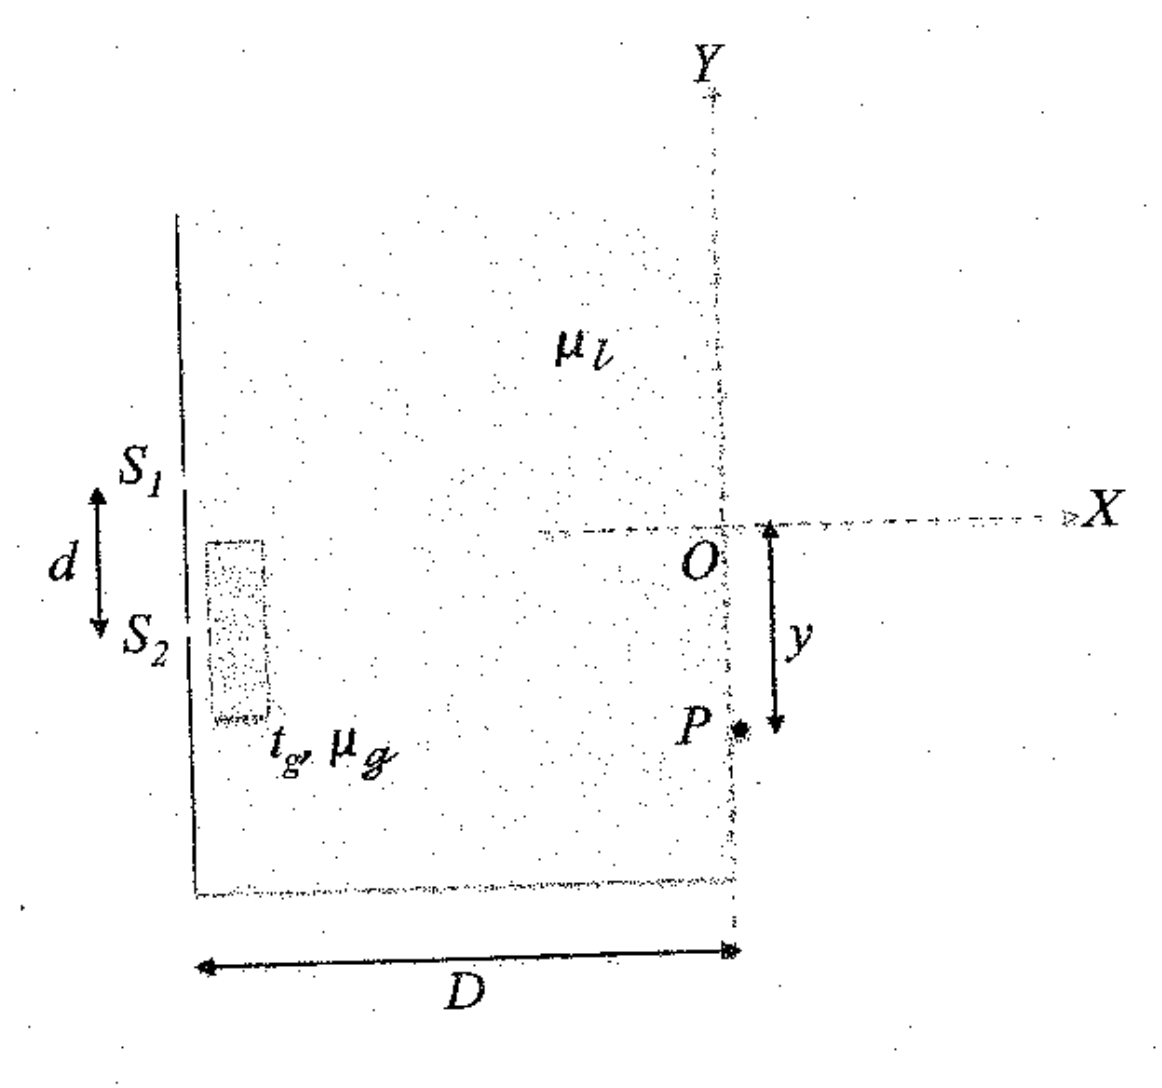
\includegraphics[width=0.5\linewidth]{spho_book_TYS_images/2012q10.png}
	\caption{Modified Young's Double Slit}
\end{figure}

(i) Consider the point $P$ on the screen at a distance $y$ from O $(S_{1} O=S_{2} O ; O P=y)$. Obtain the expression for the optical path difference $\Delta x$ in terms of the refractive indices. [3] \\
(ii) If $P$ is the central maximum. Obtain the expression for $y$ as a function of time $t$. [3] \\
(iii) Obtain the time $t_{m}$ when the central maximum is at a point $O$, equidistant from $S_{1}$ and $S_{2}$, i.e. $S_{1} O=S_{2} O$ [3] \\
(iv) Determine the speed, $v$ of the central maximum when it is at $O$. [3]
\end{document}
